\section{Hard and Hybrid Logic Networks}\label{cha:hardNetworks} % To be dropped in the unification with the MLN chapter

\red{Hard Logic Networks are Knowledge Bases, Hybrid Logic Networks are exponential families on Knowledge Bases.
This makes it impossible to build energy tensors without basemeasures capturing vanishing coordinates.}



\red{Work in Theorem~\ref{the:factorReduction} to reduce entailment!}

% Hard logic vs markov logic
While exponential families are positive distributions, in logics probability distributions can assign states zero probability.
As a consequence, Markov Logic Networks have a soft logic interpretation in the sense that violation of activated formulas have nonzero probability.
We here discuss their hard logic counterparts, where worlds not satisfying activated formulas have zero probability.

Further we investigate, how both hard and soft logic factors can be combined to hybrid networks.

%The Tensor Network decomposition of formula tensors is analogously constructed to a graphical representation of the formulas.
%We thus develop in this section the interpretation of formula tensor decompositions as Bayesian and Markov Propositional Networks.



\subsection{The limit of hard logic}\label{sec:hardLogicLimit} % To be merged with the above

The probability function of Markov Logic Networks with positive weights mimiks the tensor network representation of the knowledge base, which is the conjunction of the formulas. 
The maxima of the probability function coincide with the models of the corresponding knowledge base, if the latter is satisfiable.
However, since the Markov Logic Network is defined as a normed exponentiation of the weighted formula sum, it is a positive distribution whereas uniform distributions among the models of a knowledge base assign zero probability to world failing to be a model.
Since both distributions are tensors in the same space to a factored system, we can take the limits of large weights and observe, that Markov Logic Networks indeed converge to normed knowledge bases.


% Limit of Activation core
\begin{lemma}
	When taking the limit of large weights $\weightof{\exformula}\rightarrow\infty$ we observe a coordinatewise (in the sense of a convergence of each coordinate of the tensor) convergence 
	\begin{align}
%	\frac{1}{\partitionfunctionof{\weightof{\exformula}\exformula}} \expof{\weightof{\exformula}\exformula} 
		\normationofwrt{\expof{\weightof{\exformula}\cdot \exformula}}{\shortcatvariables}{\varnothing} \rightarrow  \normationofwrt{\exformula}{\shortcatvariables}{\varnothing}
%	\frac{1}{\braket{\exformula,\ones}}\exformula
	\end{align}
\end{lemma}
\begin{proof}
	We have 
	\begin{align*}
		\partitionfunctionof{\mlnparameters} = (\prod_{\atomenumerator} \catdimof{\atomenumerator} - \contractionof{\exformula}{\varnothing}) + \contractionof{\exformula}{\varnothing} \cdot \expof{\weightof{\exformula}}
	\end{align*}
	and therefore for any $\atomindices\in\atomstates$ with $\exformula(\atomindices)=1$
	\begin{align*}
		\normationofwrt{\expof{\weightof{\exformula}\cdot \exformula}}{\indexedcatvariables}{\varnothing} 
		&= \frac{
			\expof{\weightof{\exformula}}
			}{
			(\prod_{\atomenumerator} \catdimof{\atomenumerator} - \contractionof{\exformula}{\varnothing}) + \contractionof{\exformula}{\varnothing} \cdot \expof{\weightof{\exformula}}
			} \\
		& \rightarrow \frac{1}{\contractionof{\exformula}{\varnothing}} 
		= \normationofwrt{\exformula}{\indexedcatvariables}{\varnothing} \, . 
	\end{align*}
	For any $\atomindices\in\atomstates$ with $\exformula(\atomindices)=0$ we have on the other side
	\begin{align*}
		\normationofwrt{\expof{\weightof{\exformula}\cdot \exformula}}{\indexedcatvariables}{\varnothing} 
		&= \frac{
			1
			}{
			(\prod_{\atomenumerator} \catdimof{\atomenumerator} - \contractionof{\exformula}{\varnothing}) + \contractionof{\exformula}{\varnothing} \cdot \expof{\weightof{\exformula}}
			} \\
		& \rightarrow 0
		= \normationofwrt{\exformula}{\indexedcatvariables}{\varnothing} \, . 
	\end{align*}
\end{proof}

\begin{theorem}
	Let $\formulaset$ be a formulaset and $\canparam$ a positive parameter vector.
	If the formula
		\[ \kb = \bigwedge_{\exformulain} \exformula \]
	is satisfiable we have in the limit $\invtemp\rightarrow\infty$ the coordinatewise convergence
		\[ \expdistofat{(\formulaset,\invtemp\cdot\canparam)}{\shortcatvariables} \rightarrow \normationofwrt{\kb}{\shortcatvariables} \, . \]
\end{theorem}
\begin{proof}
	Since $\kb$ is satisfiable we find $\catindices\in\atomstates$ with
		\[  \contractionof{\expof{\sum_{\exformulain}\invtemp\cdot \weightof{\exformula} \cdot \exformula}}{\indexedcatvariables} = \expof{\invtemp \cdot \sum_{\exformulain}\weightof{\exformula}}  \]
	and the partition function obeys
		\[ \contractionof{\expof{\sum_{\exformulain}\invtemp\cdot \weightof{\exformula} \cdot \exformula}}{\varnothing} \geq  \expof{\invtemp \cdot \sum_{\exformulain}\weightof{\exformula}}  \, . \]
	For any state $\catindices\in\atomstates$ with $\kb(\catindices)=0$ we find $\secexformula\in\formulaset$ with $\secexformula(\catindices)=0$ and have
	\begin{align*}
	 	\frac{
		\contractionof{\expof{\sum_{\exformulain}\invtemp\cdot \weightof{\exformula} \cdot \exformula}}{\indexedcatvariables}
		}{
		\contractionof{\expof{\sum_{\exformulain}\invtemp\cdot \weightof{\exformula} \cdot \exformula}}{\varnothing}
		} 
		\leq  
	 	\frac{
		\expof{\invtemp\cdot \sum_{\exformulain : \exformula\neq \secexformula}\weightof{\exformula}}
		}{
		\expof{\invtemp\cdot \sum_{\exformulain}\weightof{\exformula}}
		} 
		= \expof{\invtemp \cdot \weightof{\secexformula}} \rightarrow 0 \, . 
	\end{align*}
	The limit of the distribution has thus support only on the models of $\kb$. 
	Since any model of $\kb$ has same energy at any $\invtemp$ the limit is a uniform distribution and coincides therefor with
		\[ \normationofwrt{\kb}{\shortcatvariables} \, . \]
\end{proof}


\begin{remark}[More generic situation of simulated annealing]
	The process of taking $\invtemp\rightarrow\infty$ is known as simulated annealing, see Chapter~\ref{cha:probReasoning}.
	From the discussion there we have the more general statement, that the limiting distribution is the uniform distribution among the maxima of $\expdistofat{(\formulaset,\canparam)}{\shortcatvariables}$.
	If the formula $\kb$ is not satisfiable the normation $\normationofwrt{\kb}{\shortcatvariables}{\varnothing}$ does not exist and the limit distribution has another syntactical representation, to be gained e.g. by minterm or maxterm representation (see Theorem~\ref{the:tensorToMaxMinTerms}).
\end{remark}





%To make this convergence precise, we define the uniform distribution 
%\begin{align}
%	\expdistofat{\kb}{\datapoint}
%	= \begin{cases} 
%	\frac{1}{\braket{\ftensorof{\kb},\ones}} & \text{if } \braket{\ftensorof{\kb},\datapoint} = 1 \\
%	0 &  \text{if } \braket{\ftensorof{\kb},\datapoint} = 0
%	\end{cases}
%\end{align}

%\begin{theorem}
%	Given a MLN parameterized by $\mlnparameters$, we have for $\lambda\rightarrow\infty$
%		\[ \kldivof{\expdistofat{(\formulaset,\lambda\cdot\weight)}{\datapoint}}{\expdistofat{\kb}{\datapoint}} \rightarrow 0 \, .\]
%\end{theorem}
%\begin{proof}
%	Follows directly from the convergence at each core.
%\end{proof}














\subsection{Hard Logic Networks}

Hard Logic Network coincide with Knowledge Bases.
We use $\land$ symmetry to represent them as a contraction of the formulas building the Knowledge Base as conjunction.

\begin{theorem}[Conjunction Decomposition of Knowledge Bases]\label{the:conDecKB}
	For a Knowledge Base
		\[ \kb = \bigwedge_{\exformula\in\formulaset} \exformula \]
	we have
		\[ \kbat{\shortcatvariables} = \contractionof{\formulaat{\shortcatvariables}}{\shortcatvariables}   \]
	and
		\[ \kbat{\shortcatvariables} = \contractionof{\{\rencodingofat{\exformula}{\catvariableof{\exformula},\shortcatvariables} \, : \, \exformula\in\formulaset\} \cup \{\onehotmapofat{1}{\catvariableof{\exformula}} \, : \, \exformula\in\formulaset\} }{\shortcatvariables} \, .  \]
\end{theorem}
\begin{proof}
	By the $\land$-symmetry, see effective calculus and 
		\[ \formulaat{\shortcatvariables} =  \contractionof{\{\rencodingofat{\exformula}{\catvariableof{\exformula},\shortcatvariables}, \onehotmapofat{1}{\catvariableof{\exformula}}\} }{\shortcatvariables} \]
\end{proof}

\begin{remark}{$\land$ symmetry does not generalize to Markov Logic Networks}
	% Comparison to Markov Logic
	In Markov Logic, similar decompositions are not possible.
	For example, consider a MLN with a single formula $\atomicformulaof{0}\land\atomicformulaof{1}$ and nonvanishing weight $\canparam$.
	This does not coincide with the distribution of a MLN of two formulas $\atomicformulaof{0}$ and $\atomicformulaof{1}$.
	To see this, we notice that with respect to the distribution of the first MLN, both variables are not independent, while for any MLN constructed by the two atomic formulas they are.
\end{remark}


%It is known, that there are symmetries in the syntactical represention of Knowledge Bases.
%
%There is a lot of redundancy in the activation of Knowledge Cores describing exactly the same models.
%
%\begin{theorem}[$\land$-symmetry]\label{the:landSymmetry}
%	We observe that the contraction of an $\land$ core with $\tbasis$  is equivalent with $\tbasis$ cores on all the connected subformulas.
%\end{theorem}
%\begin{proof}
%	By equality of the Knowledge Base contraction in both ways: The missing subformulas behave the same if they are activated, since they then are contrained to the same subnetworks somewhere else. 
%	%\red{Find better arguments for missing subformulas when having the larger core.}
%\end{proof}
%
%\begin{theorem}[$\lnot$-symmetry]
%	Similarly the contraction of an $\lnot$ core with $\tbasis$ or $\tbasis$ has the same result as with $\tbasis$ or $\tbasis$ on the subformula.
%\end{theorem}
%
%We call the application of these in changing the Knowledge Cores without changing the contracted network as the representation symmetry.


\subsubsection{Conjunctive Normal Representation}

\red{Poly reps here?}

We can now apply the representation symmetries to represent a propositional Knowledge Base in conjunctive normal form.
A Knowledge Base in Conjunctive Normal Form is a conjunction of clauses, where clauses are disjunctions of literals being atoms (positive literals) or negated atoms (negative literals).




%One tensor representation of a Knowledge Base is the association of the Knowledge Core $\tbasis$ at the formula being the Knowledge Base itself.
%We can use the $\land$ symmetry (Theorem~\ref{the:landSymmetry}) to propagate $\tbasis$ to all clause cores and get an alternative representation.
%Those are especially interesting when using Modus Ponens/Resolution as local sub-KB reasoners (see Section~\ref{subsec:LocalEntailment}).


\subsubsection{Polynomial Representation of Formulas}

\red{We can further derive representation schemes for Knowledge Bases, which are in conjunctive normal forms.}

Formulas can be represented as sparse polynomials, which will be discussed in more detail in Chapter~\ref{cha:sparseTC} (see Definition~\ref{def:polynomialSparsity}).

\begin{lemma}\label{lem:clauseTermBasisPlus}
	Any term is representable by a single monomial and any clause is representable by at most two monomials. %, any term of basis+ with rank 1. %Use also \baspluscprankof{}
\end{lemma}
\begin{proof}
	Let $\nodes_0$ and $\nodes_1$ be disjoint subsets of $\nodes$, then we have
	\begin{align*}
		\termof{\nodes_0}{\nodes_1} = \onehotmapofat{
			\{\catindexof{\atomenumerator} = 0 : \atomenumerator\in\nodes_0\} \cup \{\catindexof{\atomenumerator} = 1 : \atomenumerator\in\nodes_1\}
		}{\catvariableof{\nodes_0\cup\nodes_1}} \otimes \onesat{\catvariableof{\nodes/(\nodes_0\cup\nodes_1)}}
	\end{align*}
	and
	\begin{align*}
		\clauseof{\nodes_0}{\nodes_1} = \onesat{\catvariableof{\nodes}} - \onehotmapofat{
			\{\catindexof{\atomenumerator} = 0 : \atomenumerator\in\nodes_0\} \cup \{\catindexof{\atomenumerator} = 1 : \atomenumerator\in\nodes_1\}
		}{\catvariableof{\nodes_0\cup\nodes_1}}
		\otimes \onesat{\catvariableof{\nodes/(\nodes_0\cup\nodes_1)}} \, . 
	\end{align*}
	We notice, that any tensors $\ones$ and $\onehotmapof{\catindex}\otimes \ones$ habe basis+-rank of $1$ and therefore $\termof{\nodes_0}{\nodes_1}$ of $1$ and $\clauseof{\nodes_0}{\nodes_1}$ of at most $2$.
\end{proof}


We apply Lemma~\ref{lem:clauseTermBasisPlus} to show the following sparsity bound on the energy tensor of Markov Logic Networks.

\begin{theorem}
	Any formula $\exformula$ with a conjunctive normal form of $n$ clauses satisfies
		\[ \slicesparsityof{\exformula} \leq 2^{n} \, . \]
	For any set $\formulaset$ of formulas each with a conjunctive normal form of $n_{\exformula}$ clauses satisfies for any $\weight$
		\[ \slicesparsityof{\sum_{\exformulain}\weightof{\exformula}\cdot\exformula} \leq \sum_{\exformulain}2^{n_{\exformula}} \, . \]
\end{theorem}
\begin{proof}
	Let $\exformula$ have a CNF with clauses indexed by $l\in[n]$ and each clause represented by subsets $\nodes_0^l, \nodes_1^l$, that is
		\[ \exformula = \bigwedge_{l \in [n]}  \clauseof{\nodes_0^l}{\nodes_1^l} \, . \]
	We now use the rank bound of Theorem~\ref{the:CPrankContractionBound} and Lemma~\ref{lem:clauseTermBasisPlus} to get
	\begin{align*}
		\slicesparsityof{\exformula} \leq \prod_{l \in [n]}  \slicesparsityof{\clauseof{\nodes_0^l}{\nodes_1^l}} \leq 2^n \, . 
	\end{align*}
	
	Given a collection of formulas $\formulaset$, each with a CNF of $n_{\exformula}$ clauses we apply Theorem~\ref{the:CPrankSumBound} and get
	\begin{align*}
		\slicesparsityof{\sum_{\exformulain}\weightof{\exformula}\cdot\exformula} \leq \sum_{\exformulain}\slicesparsityof{\exformula} \leq \sum_{\exformulain}2^{n_{\exformula}} \, . 
	\end{align*}
\end{proof}






\subsection{Hybrid Logic Network}

Markov Logic Networks are by definition positive distributions.
In contrary, Hard Logic Networks model uniform distributions over model sets of the respective Knowledge Base and therefore have vanishing coordinates.
We now show how to combine both approaches by defining Hybrid Logic Networks.
\red{
We orient on Example 3.6 in \cite{wainwright_graphical_2008} and choose hard constraints as a base measure $\hfbasemeasure$, probabilistic soft formulas as sufficient statistics as before.
}

\begin{definition}
	Given a set of formulas $\softformulaset$ with weights $\canparam$ and set $\hardformulaset$ of formulas, which conjunction is satisfiable, the hybrid logic network is the probability distribution
	\begin{align*}
		\probtensorof{(\softformulaset,\canparam,\hfbasemeasure)}[\shortcatvariables] 
		= \normationof{
		\{\exformula : \exformula\in\hardformulaset\} \cup \{\expof{\weightof{\exformula}\cdot\exformula} : \exformula\in\softformulaset\}
		}{\shortcatvariables} \, ,
	\end{align*}
	which is the member of the exponential family with statistic by $\softformulaset$ and the base measure
		\[ \hfbasemeasure[\shortcatvariables] = \contractionof{\{\formula : \formula \in \hardformulaset\}}{\shortcatvariables} \, .\]
\end{definition}

The assumption of a satisfiable set $\hardformulaset$ is necessary, as we show next.

\begin{theorem}
	If any only if $\bigwedge_{\formula\in\hardformulaset}\formula$ is satisfiable, the tensor 
		\[  \contractionof{
		\{\exformula : \exformula\in\hardformulaset\} \cup \{\expof{\weightof{\exformula}\cdot\exformula} : \exformula\in\softformulaset\}
		}{\shortcatvariables} \]
	is normable.
\end{theorem}
\begin{proof}
	We need to show that
	\begin{align}\label{eq:tbsWellDefinedHLN}
		\contraction{\{\exformula : \exformula\in\hardformulaset\} \cup \{\expof{\weightof{\exformula}\cdot\exformula} : \exformula\in\softformulaset\}} > 0 \, . 
	\end{align}
	Since the conjunction of $\hardformulaset$ is satisfiable we find a $\shortcatindices$ with $\formulaat{\indexedcatvariableof{[\catorder]}}=1$ for all $\exformula\in\hardformulaset$.
	Then 
	\begin{align*}
		 \contractionof{\{\exformula : \exformula\in\hardformulaset\} \cup \{\expof{\weightof{\exformula}\cdot\exformula} : \exformula\in\softformulaset\}}{\indexedcatvariableof{[\catorder]}}  
		 & = \left( \prod_{\exformula\in\hardformulaset}\formulaat{\indexedcatvariableof{[\catorder]}} \right) 
		 \cdot \left( \prod_{\exformula\in\softformulaset}\expof{\weightof{\exformula}\cdot\exformula}[\indexedcatvariableof{[\catorder]}] \right) \\
		 & =  \left( \prod_{\exformula\in\softformulaset}\expof{\weightof{\exformula}\cdot\exformula}[\indexedcatvariableof{[\catorder]}] \right) \\
		 & > 0 \, . 
	\end{align*}
	Condition \eqref{eq:tbsWellDefinedHLN} follows from this and the Hybrid Logic Network is well-defined.
\end{proof}


%\subsubsection{Representation as Exponential Families}

%We call graphical models which contain cores from a Markov Logik Network and of a Hard Logic Network a Hybrid Logic Network.

%Hybrid logic networks are exponential family, where the hard logic factors build a base measure and the probabilistic logic components a contracted statistics function.
%\begin{theorem}
%	A hybrid logic network $\probtensorof{(\softformulaset,\canparam,\hardformulaset)}$ is in the exponential family with base measure
%		\[ \hfbasemeasure[\shortcatvariables] = \contractionof{\{\formula : \formula \in \hardformulaset\}}{\shortcatvariables} \] % Do not need a normed base measure!
%	and sufficient statistic $\softformulaset$ the element with parameters $\canparam$.
%\end{theorem}

%
%By a slight abuse of notation, we denote by $\hardformulaset$ both the set of propositional formulas and their contractions.



\subsubsection{Tensor Network Representation}


We can employ the formula decompositions to represent both probabilistic facts of the MLN and hard facts (seen as the limit of large weights).

\begin{theorem}\label{the:hybridNetworkRepresentation}
	For any hybrid logic network we have
	\begin{align*}
		\probtensorof{(\softformulaset,\canparam,\hardformulaset)}[\shortcatvariables] 
		= \normationof{
		\{\rencodingofat{\exformula}{\catvariableof{\exformula},\shortcatvariables} : \exformula\in\softformulaset\cup\hardformulaset \}
		\cup \{\onehotmapofat{1}{\catvariableof{\exformula}} : \exformula\in\hardformulaset \}
		\cup \{\headcoreofat{\exformula}{\catvariableof{\exformula}} : \exformula\in\softformulaset \}
		}{\shortcatvariables} \, . 
	\end{align*}
\end{theorem}
\begin{proof}
	By Lemma~\ref{lem:formulaEncodingDecomposition}.
\end{proof}

%% Overwork: Allow for infinite weights?
%Capturing hard and soft constraints at the same time, we can use a weight to each formula:
%\begin{itemize}
%	\item $\weightof{\exformula}=0$: The formula is neutral and does not influence the probability distribution.
%	Techniacally, the formula tensor is contracted with a $\ones$ head with the result being a $\ones$ world tensor, which leaves other products invariant under Hadamard products.
%	\item $\weightof{\exformula}=\infty$: The formula is a hard constraint. 
%	\item $\weightof{\exformula} \in (0,\infty)$: The fromula is a probabilistic constraint.
%\end{itemize}



%The reason for this is the Slicing Theorem, enabling the operations by both (exponentiation and selection of one slice) by the head cores.
For an example see Figure~\ref{fig:ActivatedHeads}.

\begin{figure}[h]
\begin{center}
	\begin{tikzpicture}[scale=0.35, thick, yscale=-1] % , baseline = -3.5pt


\draw[<-] (0,-1)--(0,1) node[midway,left] {\tiny $\catvariableof{a}$}; 
\draw[<-] (1.5,-1)--(1.5,1) node[midway,right] {\tiny $\catvariableof{b}$}; 
\draw[<-] (3,-1)--(3,1) node[midway,right] {\tiny $\catvariableof{c}$}; 
\draw (-1,-1) rectangle (4, -3);
\node[anchor=center] (text) at (1.5,-2) {$\partitionfunction \cdot \probtensor$};



\node[anchor=center] (text) at (5.5,-2) {${=}$};


\begin{scope}[shift={(11,0)}]

\draw[->] (0,1)--(0,-1)  node[midway,left] {\tiny $\catvariableof{a}$}; 
\draw[->]  (3,1)--(3,-1) node[midway,right] {\tiny $\catvariableof{b}$}; 
\draw[->] (6,1)--(6,-1) node[midway,right] {\tiny $\catvariableof{c}$}; 
	
\draw (-1,-1) rectangle (4, -3);
\node[anchor=center] (text) at (1.5,-2) {$\concoreof{\lor}$};

\draw[->] (1.5,-3) --(1.5,-4.5) node[midway,right]{\tiny $\catvariableof{a \lor b}$};
\drawvariabledot{1.5}{-4.5}
\draw[->] (1.5,-4.5) --(1.5,-6) ;


\draw[fill, \probcolor] (1.5,-4.5) circle (0.15cm);
\draw[\probcolor] (1.5,-4.5) -- (-0.25,-4.5);
\draw[\probcolor]  (-6.75, -3.5) rectangle (-0.25, -6.5);
\node[anchor=center,\probcolor] (text) at (-3.5,-5) {$\begin{bmatrix} 
1 \\
\expof{\canparam}
\end{bmatrix}$};

\draw (5,-1) rectangle (7, -3);
\node[anchor=center] (text) at (6,-2) {$\concoreof{\lnot}$};

\draw[->] (6,-3) --(6,-4.5) node[midway,right]{\tiny $\catvariableof{\lnot c}$};
\drawvariabledot{6}{-4.5}
\draw[->] (6,-4.5) --(6,-6);	


	
\draw (0.5,-6) rectangle (6.5,-8);
\node[anchor=center] (text) at (3.5,-7) {$\concoreof{\lor}$};
	
\draw[<-] (4,-9.5) -- (4,-8) node[midway,right] {\tiny $\catvariableof{a \lor b \lor \lnot c}$};

\draw[fill,\concolor] (4,-9.5) circle (0.15cm);
\draw[\concolor] (4,-9.5) -- (2.25,-9.5);
\draw[\concolor]  (0.25, -8.5) rectangle (2.25, -11.5);
\node[anchor=center,\concolor] (text) at (1.25,-10) {$\begin{bmatrix} 
0 \\
1
\end{bmatrix}$};

%\draw (3,-9) rectangle (5,-11);
%\node[anchor=center] (text) at (4,-10) {$\truevectorat{}$};

\end{scope}

\end{tikzpicture}
\end{center}
\caption{Diagram of a formula tensor with activated heads, containing \textcolor{\concolor}{hard constraint cores} and \textcolor{\probcolor}{probabilistic weight cores} .} %along \textcolor{\inactivecolor}{inactive cores}.}
\label{fig:ActivatedHeads} 
\end{figure}



\begin{remark}{Probability interpretation using the Partition function}
	The tensor networks here represent unnormalized probability distributions.
	The probability distribution can be normed by the quotient with the naive contraction of the network, the partition function.
\end{remark}


\subsubsection{Reasoning Properties}



\begin{theorem}
	Let $(\softformulaset,\canparam,\hardformulaset)$ define a Hybrid Logic Network.
	Given a query formula $\exformula$ we have that 
		\[ \probtensorof{(\softformulaset,\canparam,\hardformulaset)} \models \exformula \]
	if and only if
		\[ \hardformulaset \models \exformula \, . \]
\end{theorem}
\begin{proof}
	Application of Theorem~\ref{the:factorReduction} on the representation of Hybrid Logic Networks as Markov Networks in Theorem~\ref{the:hybridNetworkRepresentation}.
\end{proof}


%% Now in theorems
%\begin{itemize}
%	\item Entailment queries answered on the hard logic parts alone.
%	\item Well defined distributions, when hard logic formulas are satisfiable.
%	\item Redundant hard formulas (Redundancy, whenever the contractions unchanged): If entailled by the rest of the hard logic formulas. 
%	\item Redundant soft formulas (Redundancy, whenever the normations unchanged):  Either if entailled or contradicted by the hard logic formulas
%\end{itemize}



Formulas in $\softformulaset$, which are entailed or contradicted by $\hardformulaset$ are redundant 

\begin{theorem}
	If for a formula $\exformula$ and $\hardformulaset$ we have  %and only if
		\[ \hardformulaset \models \exformula \, \quad \text{or} \quad \hardformulaset \models \lnot\exformula \]
	then for any $(\softformulaset,\canparam,\hardformulaset)$
		\[ \probofat{(\softformulaset/\{\exformula\},\tilde{\canparam},\hardformulaset)}{\shortcatvariables} =  \probofat{(\softformulaset,\canparam,\hardformulaset)}{\shortcatvariables}  \, , \]
	where $\tilde{\canparam}$ denotes the tensor $\canparam$, where the coordinate to $\exformula$ is dropped, if $\exformula\in\softformulaset$.
\end{theorem}
\begin{proof}
	Isolate the factor to the hard formula, which is constant for all situations.
\end{proof}

%% Now in the 
A similar statement holds for the hard formulas itself, as shown in Theorem~\ref{the:ReduncancyOfEntailed}.
However, notice that if $\hardformulaset/\{\exformula\}\models\lnot\exformula$, then $\hardformulaset\cup\{\exformula\}$ is not satisfiable and a hybrid logic network cannot be defined for $\hardformulaset\cup\{\exformula\}$ as hard logic formulas.

%If the conjunction of $\hardformulaset/\{\exformula\}$ entails $\exformula$, we can erase $\exformula$ from $\hardformulaset$ without changing the contraction, therefore without changing the base measure of the Hybrid Logic Network.



\subsubsection{Expressivity}

Hybrid Logic Networks extend the expressivity result of Theorem~\ref{the:mintermExpressivityMLN} to arbitrary probability tensors, dropping the positivity constraints for Markov Logic Networks.

\begin{theorem}\label{the:mintermExpressivityHLN}
	Let $\probat{\shortcatvariables}$ a possibly not positive probability tensor we build a base measure
		\[ \hfbasemeasure = \nonzeroof{\probat{\shortcatvariables}} \]
	and a parameter tensor
	\begin{align*}
		\canparamat{\selvariableof{[\catorder]}=\shortcatindices}
		= \begin{cases}
			0 & \text{if} \quad \probat{\shortcatvariables=\shortcatindices} = 0  \\
			\lnof{\probat{\shortcatvariables=\shortcatindices}} & \text{else} 
		\end{cases} \, . 
	\end{align*}
	Then the probability tensor is the member of the minterm exponential family with base measure $\hardformulaset$ and parameter $\canparam$, that is
		\[ \probof{(\mintermformulaset,\canparam,\hfbasemeasure)}\]
\end{theorem}
\begin{proof}
	It suffices to show that 
		\[ \sbcontractionof{\hfbasemeasure, \expof{\contractionof{
		\sencodingof{\mintermformulaset}\canparam
		}{
		\shortcatvariables
		}}}{\shortcatvariables} = \probat{\shortcatvariables} \, . \]
	For indices $\shortcatindices$ with $\probat{\shortcatvariables=\shortcatindices}=0$ we have $\hfbasemeasureat{\shortcatvariables=\shortcatindices}=0$ and thus also 
		\[ \sbcontractionof{\hfbasemeasure, \expof{\contractionof{
		\sencodingof{\mintermformulaset}\canparam
		}{
		\shortcatvariables
		}}}{\shortcatvariables=\shortcatindices} = 0 \, . \]
	For indices $\shortcatindices$ with $\probat{\shortcatvariables=\shortcatindices}>0$ we have $\hfbasemeasureat{\shortcatvariables=\shortcatindices}=1$ and
	\begin{align*}
		 \sbcontractionof{\hfbasemeasure, \expof{\contractionof{
		\sencodingof{\mintermformulaset}\canparam
		}{
		\shortcatvariables
		}}}{\shortcatvariables=\shortcatindices} 
		&= \prod_{\selindexof{[\catorder]}} \expof{\canparamat{\selvariableof{[\catorder]}=\selindexof{[\catorder]}} \cdot \mintermofat{\selindexof{[\catorder]}}{\shortcatvariables=\shortcatindices}} \\
		&=  \expof{\canparamat{\selvariableof{[\catorder]}=\shortcatindices}} \\
		&=  \probat{\shortcatvariables=\shortcatindices} \, .
	\end{align*}
\end{proof}




\subsection{Categorical Constraints}\label{sec:categoricalTN}

\red{Also called atomization of categorical variables.}

%% Categorical variables with more possibilities
We made the assumption that all categorical variables in factored systems to be represented by propositional logics take binary values (i.e. $\catdim=2$).
In cases where a categorical variable $\catvariable$ takes multiple values we define for each $\catindex$ an atomic formula $\catvariableof{\catindex}$ representing whether $\catvariable$ is assigned by $\catindex$ in a specific state.
	%\[ \catvariableof{\catindex} =  (\catvariable = \catindex \, . \] Confusing notation
Following this construction we have the constraint that exactly one of the atoms $\catvariableof{\catindex}$ is $1$ at each state.

%% Capture constraint
To capture the constraints resulting from this construction we introduce auxiliary parts. % of Bayesian Propositional Networks.
Such constraints can also be expressed by a formula but would result in an unnecessary large tensor network.


%% Categorical selection map
\begin{definition}[Categorical Constraint]
	Given a list $\catvariableof{0},\ldots,\catvariableof{\catdim-1}$ of binary variables and a categorical variable $\catvariable$ with dimension $\catdim$ a categorical constraint is a tensor $\categoricalmap[\catvariable,\catvariableof{[\catdim]}]$ defined as
%	A categorical constraint taking values in $[\catdim]$ maps to its atoms by
%		\[ \categoricalmap : [\catdim] \rightarrow \bigtimes_{\catindex\in[\catdim]}[2]  \]
	\begin{align*}
		 \categoricalmap(\catindex,\catindexof{\variableset}) 
		 = \begin{cases} 
		 	1 & \text{if} \quad \catindexof{[\catdim]} = \onehotmapof{\catindex} \\
			0 & \text{else} \, . 
		 \end{cases}
	\end{align*}
% where the $1$ is at position $\catindex$.
\end{definition}

%% Decomposition
With Theorem~\ref{the:functionDecompositionBasisCP} the tensor representation of $\categoricalcore$ decomposes in a basis CP format (see Figure~\ref{fig:CategoricalDecomposition}b) of if its coordinate maps $\categoricalmap_{\catindex}$, where $\catindex\in[\catdim]$.
For the cores
\begin{align}
	\categoricalcoreof{\catindex} = \onehotmapofat{\catindex}{\catvariable} \otimes \onehotmapofat{1}{\catvariableof{\catindex}} + (\onesat{\catvariable}- \onehotmapofat{\catindex}{\catvariable} ) \otimes \onehotmapofat{0}{\catvariableof{\catindex}} 
\end{align}	
we have by Theorem~\ref{the:functionDecompositionBasisCP}
\begin{align*}
	\rencodingofat{\categoricalmap}{\catvariable, \catvariableof{0}, \ldots, \catvariableof{\catdim-1}} 
	= \contractionof{\{\rencodingof{\categoricalmap(\catindex)} \, : \, \catindex\in[\catdim]\}}{\catvariable, \catvariableof{0}, \ldots, \catvariableof{\catdim-1}} \, . 
\end{align*}


In the next theorem we show how a categorical constraint can be enforced in a tensor network by adding the tensor $\categoricalmap$ to a contraction.

\begin{theorem}
	For any tensor $\hypercoreat{\shortcatvariables}$ and a categorical constraint defined by an ordered subset $\catvariableof{\variableset}\subset\shortcatvariables$, a variable $\catvariable\in\shortcatvariables$ we have
	\begin{align*}
	 	\contractionof{\{\hypercoreat{\shortcatvariables}, \categoricalmap\}}{\indexedcatvariables} 
		= \begin{cases}
			\hypercoreat{\indexedcatvariables} & \text{if} \quad \catindexof{\variableset} = \onehotmapof{\catindex} \\
			0 & \text{else} \, . 
		\end{cases}
	\end{align*}
\end{theorem}
\begin{proof}
	For any $\catindexof{[\atomorder]}$ we have
		\[ \contractionof{\{\hypercoreat{\shortcatvariables}, \categoricalmap\}}{\indexedcatvariables}  = 
			\hypercoreat{\indexedcatvariableof{[\atomorder]}} \cdot \categoricalmap[\indexedcatvariableof{},\indexedcatvariableof{\variableset}] \, . 
		\]
	If $\catindexof{\variableset} = \onehotmapof{\catindex}$ we have $\categoricalmap[\indexedcatvariableof{},\indexedcatvariableof{\variableset}] = 1$ and thus
		\[ \contractionof{\{\hypercoreat{\shortcatvariables}, \categoricalmap\}}{\indexedcatvariables}  =  \hypercoreat{\indexedcatvariableof{[\atomorder]}}  \, . \]
	If $\catindexof{\variableset} \neq \onehotmapof{\catindex}$ then $\categoricalmap[\indexedcatvariableof{},\indexedcatvariableof{\variableset}] = 0$ and  
		\[ \contractionof{\{\hypercoreat{\shortcatvariables}, \categoricalmap\}}{\indexedcatvariables}  = 0 \, . \]
\end{proof}




%We define the corresponding network cores as
%\begin{align}
%	\categoricalcoreof{\catindex} =
%	\begin{cases}
%		\tbasis & \text{ if } \catvariable = \catindex \\
% 		\fbasis & \text{ else }
%	\end{cases} \, . 
%\end{align}	

%Similar to atom selector tensor, but different core definition ($\fbasis$ instead of $\ones$, when $\parindexof{}$ is not matching the core position).

%% CONFUSING!
%We represent the categorical constraint as another variable $\randomxof{\categoricalmap}$, which when known defines the values of the corresponding variables $\randomxof{\atomenumerator}$ (see Figure~\ref{fig:CategoricalDecomposition}a).


\begin{figure}[h]
\begin{center}
	\begin{tikzpicture}[scale=0.35, thick] % , baseline = -3.5pt

\begin{scope}[shift={(-15,2)}]

\node[anchor=center] (text) at (-1,3) {${a)}$};


\node [circle, draw, thick, fill=gray!50] (T1) at (0,0) {\tiny $\randomxof{0}$};	
\node [circle, draw, thick, fill=gray!50] (T2) at (3,0) {\tiny $\randomxof{1}$};	
\node[anchor=center] (text) at (6,0) {\small $\cdots$};
\node [circle, draw, thick, fill=gray!50] (T3) at (9,0) {\tiny $\randomxof{\atomorder-1}$};	

\node [circle, draw, thick, fill=gray!50] (C) at (4.5,-5) {\tiny $\randomxof{\categoricalmap}$};	

\draw[->] (C) -- (T1);
\draw[->] (C) -- (T2);
\draw[->] (C) -- (T3);

\end{scope}

\node[anchor=center] (text) at (-1,5) {${b)}$};


\drawatomindices{0}{2}
\draw (-1,1) rectangle (5,-1);
\node[anchor=center] (text) at (2,0) {\small $\categoricalcore$};
\draw[->] (2,-3) -- (2,-1) node[midway,left] {\tiny $\randomxof{\categoricalmap}$};

\node[anchor=center] (text) at (7,0) {${=}$};


\begin{scope}[shift={(10,2)}]

\newcommand{\conposseldec}{4.5,-5.5}

\draw[fill] (\conposseldec) circle (0.25cm);
\draw (\conposseldec) -- (4.5,-7.5) node[midway, right] {\tiny $\randomxof{\categoricalmap}$};
%!TEX encoding = UTF-8 Unicode\draw[dashed] (3.5,-7.5) rectangle (5.5, -9.5);
%\node[anchor=center] (text) at (4.5,-8.5) {\small $\ones$};

\draw[<-] (0,1) -- (0,-1) node[midway,left] {\tiny $\randomxof{0}$};
\draw (-1,-1) rectangle (1, -3);
\node[anchor=center] (text) at (0,-2) {\small $\categoricalcoreof{0}$};
\draw[<-] (0,-3) to[bend right=20] (\conposseldec);


\draw[<-] (3,1) -- (3,-1) node[midway,left] {\tiny $\randomxof{1}$};
\draw (2,-1) rectangle (4, -3);
\node[anchor=center] (text) at (3,-2) {\small $\categoricalcoreof{1}$};
\draw[<-] (3,-3) to[bend right=20]  (\conposseldec);

\node[anchor=center] (text) at (6,-2) {$\cdots$};

\draw[<-] (9,1) -- (9,-1) node[midway,left] {\tiny $\randomxof{\atomorder-1}$};
\draw (7.75,-1) rectangle (10.25, -3);
\node[anchor=center] (text) at (9,-2) {\small $\categoricalcoreof{\atomorder-1}$};
\draw[<-] (9,-3) to[bend left=20]  (\conposseldec);




\end{scope}

		


\end{tikzpicture}
\end{center}
\caption{Representation of a categorical constraint in a $\cpformat$ Format tensor network.
	a) Representation of the dependency of the graphical model.
	b) Tensor Representation with further network decomposition.
	We average by contraction with the dashed tensor $\ones$, if we do not specify the active atom.
	}
\label{fig:CategoricalDecomposition}
\end{figure}

\begin{remark}[Combination of Constraints]
	We can combine constraint cores by Hadamard products in the dual tensor network representation, as long as they can be satisfied together.
	An example, where this is not the case, are the categorical constraints to the three sets
		\[ \{\randomxof{0},\randomxof{1},\randomxof{2},\randomxof{3}\} \, , \, \{\randomxof{0},\randomxof{1}\}\, ,\,\{\randomxof{2},\randomxof{3}\} \, . \] 
	Besides the categorical cores also the datacores have a similar bayesian network affecting the atoms by another hidden variable.
	Combining both is welldefined, only when all datapoints satisfy the categorical constraints (that is only one of the atoms in each constraint is active).
\end{remark}


\begin{example}[Sudoku]
	An interesting example, where categorical constraints are combined is Sudoku, the game of assigning numbers to a grid.
	For a $n\in\nn$ we define variables $\catvariableof{i,j,k}$ where $i,j,k\in[n^2]$ and $\catdimof{i,j,k}=2$.
	By understanding $i$ as a line index and $j$ as a column index, they are ordered in a grid as sketched in Figure~\ref{fig:sudokuGrid} in the case $n=3$.
	
%	We further define atomization variables
%		\[ \catvariableof{i,j,k} = (\catvariableof{i,j} == k) \, . \]
%	\red{These are also at each $i,j$ categorical constraints!}
	
	
	At each position there is a single number, that is for each $i,j\in[n^2]$ have a constraint
		\[ \{\catvariableof{i,j,k} \, : \, k \in [n^2] \} \]
	
	Here the $n^6$ variables are the random variables whether a specific position has a specific number assigned.
	The $3\cdot n^2$ constraints are 
	\begin{itemize}
		\item Each number $k$ appears exactly once in each row $i\in[n^2]$:
			\[ \{\catvariableof{i,j,k}  \, : \, j \in [n^2] \} \]
		\item Each number $k$ appears exactly once in each column $j\in[n^2]$:
			\[ \{\catvariableof{i,j,k}  \, : \, i \in [n^2] \} \]
		\item Each number appears exactly once in each square $s,r\in[n]$
			\[ \{\catvariableof{i+n\cdot s,j+n\cdot r,k}  \, : \, i,j \in [n] \} \]
	\end{itemize}
	
	In total we have $3\cdot n^2 + n^4$ constraints for $n^6$ variables.

	\begin{figure}\label{fig:sudokuGrid} % ! Still without k index of the variables.
	\begin{center}
		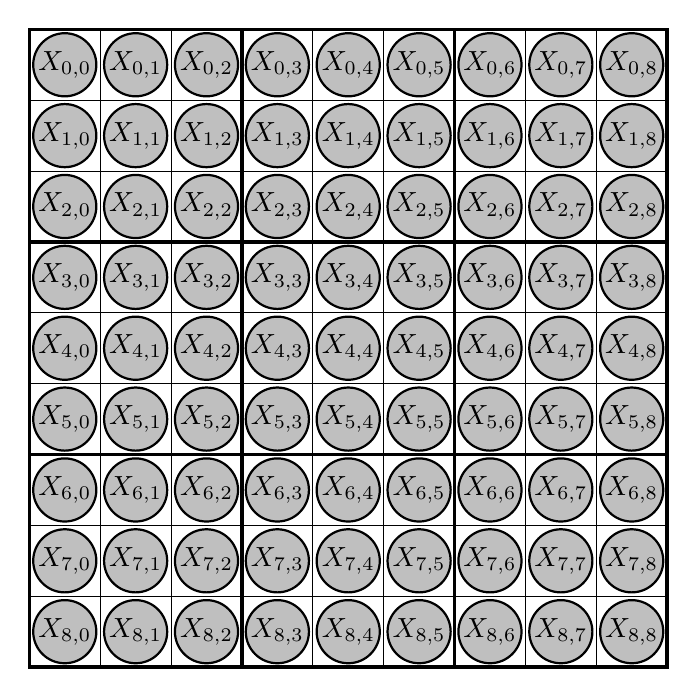
\begin{tikzpicture}[scale=0.9]
% Draw the main grid

%\node[anchor=center] (text) at (0,9) {${a)}$};

\draw[very thick] (0,0) rectangle (9,9); % Outer border
\foreach \x in {1,2,...,8} {
    \draw[thin] (\x,0) -- (\x,9); % Vertical lines
    \draw[thin] (0,\x) -- (9,\x); % Horizontal lines
}
% Thicker lines for 3x3 subgrids
\foreach \x in {3,6} {
    \draw[very thick] (\x,0) -- (\x,9); % Vertical thick lines
    \draw[very thick] (0,\x) -- (9,\x); % Horizontal thick lines
}

% Add variables in the middle of each square
\foreach \i in {0,1,...,8} {
    \foreach \j in {0,1,...,8} {
        \node[circle, draw, thick, fill=gray!50, inner sep = 0.5pt, minimum size=0.6cm, align=center] 
        at (\j+0.5,8-\i+0.5) {$X_{\i,\j}$};
    }
}

%\begin{scope}[shift={(2,0)}]
%
%\node[anchor=center] (text) at (9,9) {${b)}$};
%	
%% Draw a line of variables (horizontal)
%\foreach \k in {0,1,...,8} {
%    \node[circle, draw, thick,  fill=gray!50, inner sep=0pt, 
%    minimum size=0.6cm, align=center] 
%    at (10+\k,8.5) {$X_{i,\k}$};
%}
%
%\node[anchor=center] (text) at (9,7) {${c)}$};
%
%% Draw a column of variables (vertical)
%\foreach \l in {0,1,...,8} {
%    \node[circle, draw, thick, fill=gray!50, inner sep=0pt, 
%    minimum size=0.6cm, align=center] 
%    at (10,-\l+6) {$X_{\l,j}$};
%}
%
%\node[anchor=center] (text) at (9,7) {${d)}$};
%
%% Draw a square of variables (3x3)
%\foreach \i in {0,1,2} {
%    \foreach \j in {0,1,2} {
%        \node[circle, draw, thick, fill=gray!50, inner sep=0pt, 
%        minimum size=0.6cm, align=center] 
%        at (12+\j,6-\i) {$X_{\i,\j}$};
%    }
%}
%
%\end{scope}

\end{tikzpicture}

	\end{center}
	\caption{Sudoku grid of categorical variables, here drawn in the standard case of $n=3$, each with dimension $\catdim=n^2=9$.}
	\end{figure}

	\red{Reasoning by Entailment propagation! 
	Also, probabilistic choices possible when exact (!) contraction at a position not a basis vector, then can choose one possibility.}

\end{example}













